
%(BEGIN_QUESTION)
% Copyright 2014, Tony R. Kuphaldt, released under the Creative Commons Attribution License (v 1.0)
% This means you may do almost anything with this work of mine, so long as you give me proper credit

\noindent
{\bf Labøvelse -- introduksjon}

\vskip 5pt

Oppgaven din er å designe og bygge et analogt voltmeter med flere måleområder. Prosjektet baseres på en D'Arsonval-målemekanisme, med seriekoblede ``range''-motstander dimensjonert slik at instrumentet går nøyaktig til full skala ved forventet spenning på testledningene:

$$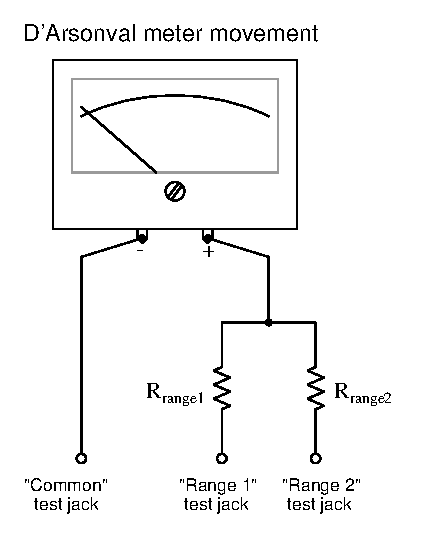
\includegraphics[width=15.5cm]{i00874x01.eps}$$

Målemekanismen alene er for følsom til å kobles direkte til en større spenningskilde. Formålet med hver område-motstand er å gi riktig totalresistans slik at instrumentnålen går til full skala ved en større og presis spenning på testjakkene. For eksempel kan måleverket ditt nå full skala med bare noen tidels volt direkte på terminalene, men med riktig område-motstand kan du få full skala ved for eksempel 10.0 V eller 50.0 V.

Hvis måleskalaen allerede har tall (f.eks. 0 til 60), bør du utnytte disse ved valg av spenningsområder (f.eks. 0 til 60 V og/eller 0 til 6.0 V).

\vskip 10pt

\filbreak

I design og bygging av prosjektet må du løse flere utfordringer. Fullføring av labøvelsen innebærer at du løser følgende utfordringer og forklarer løsningene i detalj:

\begin{itemize}
\item{} Bestemme nøyaktig fullskala-verdi for måleverket uten å overbelaste det (dvs. få nålen til å {\it slå i stopper} opp eller ned).
\item{} Bestemme nøyaktig internresistans i måleverket.
\item{} Beregne riktige område-motstander.
\item{} Finne presise område-motstander (eller bygge serie-/parallellnettverk for å oppnå ønsket motstandsverdi) for hvert område.
\item{} Identifisere metoder for justerbar kalibrering, slik at voltmeteret kan rekalibreres senere for best mulig nøyaktighet.
\item{} Finne metode for å teste voltmeteret og dokumentere nøyaktigheten.
\end{itemize}

Det forventes at du arbeider selvstendig i prosjektet, finner svar og løser problemer på egen hånd. Det er greit å utveksle ideer med medstudenter, men ikke å få andre til å løse oppgaven for deg.

Læreren er en ressurs som kan hjelpe med å avdekke misforståelser, peke på nyttige kilder og ivareta sikkerhet i laben. Det er derimot ikke lærerens oppgave å besvare tekniske spørsmål du selv kan og bør undersøke. Et overordnet formål med denne labøvelsen er å utvikle problemløsningsferdigheter og gode arbeidsvaner.

\underbar{file i00874}
%(END_QUESTION)





%(BEGIN_ANSWER)


%(END_ANSWER)





%(BEGIN_NOTES)


%INDEX% Lab exercise, building an analog voltmeter

%(END_NOTES)
